% Sample of a report for an attack as requested at wednesday, 5 December 2018, mail "Assignemnt Lab 19"
\subsection{SYN Flood}
% SCAPY program
\subsubsection{SCAPY program}
\lstinputlisting{scapy/SYNFlood.py}
With this program we are going to send every 5 milliseconds a SYN packet to an active port of the victim that we have found in the reconnaissance, in our case its port 80. \\
We have to wait that the session table of the victim reaches its edge, at this point the victim can no longer accept connections even if it is a legit ones.\par
I’ve also set the following settings on the victim pc to fill faster the session table:\\
\begin{lstlisting}
sysctl -w net.ipv4.tcp_syncookies=0
systcl -w net.ipv4.tcp_max_syn_backlog=256
\end{lstlisting}

% Wireshark presenting  the attacker's messages
\subsubsection{Victim's messages}

\begin{longtable}{|l|l|l|l|l|l|p{5cm}|}
\hline
\textbf{No.} & \textbf{Time} & \textbf{Source} & \textbf{Destination} & \textbf{Protocol} & \textbf{Length} & \textbf{Info} \\
\hline
\endhead
1 & 0.000000000 & 192.168.62.20 & 192.168.40.50 & TCP & 62 & 1024 $>$ http [SYN] Seq=0 Win=8192 Len=0 \\
\hline
2 & 0.000039000 & 192.168.40.50 & 192.168.62.20 & TCP & 56 & http $>$ 1024 [RST, ACK] Seq=1 Ack=1 Win=0 Len=0 \\
\hline
3 & 0.071742000 & 192.168.62.20 & 192.168.40.50 & TCP & 62 & blackjack $>$ http [SYN] Seq=0 Win=8192 Len=0 \\
\hline
4 & 0.071753000 & 192.168.40.50 & 192.168.62.20 & TCP & 56 & http $>$ blackjack [RST, ACK] Seq=1 Ack=1 Win=0 Len=0 \\
\hline
5 & 0.176475000 & 192.168.62.20 & 192.168.40.50 & TCP & 62 & cap $>$ http [SYN] Seq=0 Win=8192 Len=0 \\
\hline
6 & 0.176487000 & 192.168.40.50 & 192.168.62.20 & TCP & 56 & http $>$ cap [RST, ACK] Seq=1 Ack=1 Win=0 Len=0 \\
\hline
7 & 0.341383000 & 192.168.62.20 & 192.168.40.50 & TCP & 62 & 1027 $>$ http [SYN] Seq=0 Win=8192 Len=0 \\
\hline
8 & 0.341394000 & 192.168.40.50 & 192.168.62.20 & TCP & 56 & http $>$ 1027 [RST, ACK] Seq=1 Ack=1 Win=0 Len=0 \\
\hline
9 & 0.528307000 & 192.168.62.20 & 192.168.40.50 & TCP & 62 & 1028 $>$ http [SYN] Seq=0 Win=8192 Len=0 \\
\hline
10 & 0.528307000 & 192.168.40.50 & 192.168.62.20 & TCP & 56 & http $>$ 1028 [RST, ACK] Seq=1 Ack=1 Win=0 Len=0 \\
\hline
11 & 0.624187000 & 192.168.62.20 & 192.168.40.50 & TCP & 62 & solid-mux $>$ http [SYN] Seq=0 Win=8192 Len=0 \\
\hline
12 & 0.624200000 & 192.168.40.50 & 192.168.62.20 & TCP & 56 & http $>$ solid-mux [RST, ACK] Seq=1 Ack=1 Win=0 Len=0 \\
\hline
13 & 0.752630000 & 192.168.62.20 & 192.168.40.50 & TCP & 62 & 1030 $>$ http [SYN] Seq=0 Win=8192 Len=0 \\
\hline
14 & 0.752642000 & 192.168.40.50 & 192.168.62.20 & TCP & 56 & http $>$ 1030 [RST, ACK] Seq=1 Ack=1 Win=0 Len=0 \\
\hline
15 & 0.849028000 & 192.168.62.20 & 192.168.40.50 & TCP & 62 & 1031 $>$ http [SYN] Seq=0 Win=8192 Len=0 \\
\hline
16 & 0.849041000 & 192.168.40.50 & 192.168.62.20 & TCP & 56 & http $>$ 1031 [RST, ACK] Seq=1 Ack=1 Win=0 Len=0 \\
\hline
17 & 0.940368000 & 192.168.62.20 & 192.168.40.50 & TCP & 62 & 1032 $>$ http [SYN] Seq=0 Win=8192 Len=0 \\
\hline
18 & 0.940384000 & 192.168.40.50 & 192.168.62.20 & TCP & 56 & http $>$ 1032 [RST, ACK] Seq=1 Ack=1 Win=0 Len=0 \\
\hline
19 & 1.024068000 & 192.168.62.20 & 192.168.40.50 & TCP & 62 & netinfo-local $>$ http [SYN] Seq=0 Win=8192 Len=0 \\
\hline
20 & 1.024081000 & 192.168.40.50 & 192.168.62.20 & TCP & 56 & http $>$ netinfo-local [RST, ACK] Seq=1 Ack=1 Win=0 Len=0 \\
\hline
21 & 1.128540000 & 192.168.62.20 & 192.168.40.50 & TCP & 62 & activesync $>$ http [SYN] Seq=0 Win=8192 Len=0 \\
\hline
22 & 1.128556000 & 192.168.40.50 & 192.168.62.20 & TCP & 56 & http $>$ activesync [RST, ACK] Seq=1 Ack=1 Win=0 Len=0 \\
\hline
\multicolumn{7}{l}{\textit{*********************************}} \\
\hline
134 & 7.833868000 & 192.168.62.20 & 192.168.40.50 & TCP & 62 & webobjects $>$ http [SYN] Seq=0 Win=8192 Len=0 \\
\hline
135 & 7.833880000 & 192.168.40.50 & 192.168.62.20 & TCP & 56 & http $>$ webobjects [RST, ACK] Seq=1 Ack=1 Win=0 Len=0 \\
\hline
136 & 7.941336000 & 192.168.62.20 & 192.168.40.50 & TCP & 62 & cplscrambler-lg $>$ http [SYN] Seq=0 Win=8192 Len=0 \\
\hline
137 & 7.941351000 & 192.168.40.50 & 192.168.62.20 & TCP & 56 & http $>$ cplscrambler-lg [RST, ACK] Seq=1 Ack=1 Win=0 Len=0 \\
\hline
138 & 8.036353000 & 192.168.62.20 & 192.168.40.50 & TCP & 62 & cplscrambler-in $>$ http [SYN] Seq=0 Win=8192 Len=0 \\
\hline
139 & 8.036366000 & 192.168.40.50 & 192.168.62.20 & TCP & 56 & http $>$ cplscrambler-in [RST, ACK] Seq=1 Ack=1 Win=0 Len=0 \\
\hline
140 & 8.092614000 & 192.168.62.20 & 192.168.40.50 & TCP & 62 & cplscrambler-al $>$ http [SYN] Seq=0 Win=8192 Len=0 \\
\hline
141 & 8.092628000 & 192.168.40.50 & 192.168.62.20 & TCP & 56 & http $>$ cplscrambler-al [RST, ACK] Seq=1 Ack=1 Win=0 Len=0 \\
\hline
142 & 8.191949000 & 192.168.62.20 & 192.168.40.50 & TCP & 62 & ff-annunc $>$ http [SYN] Seq=0 Win=8192 Len=0 \\
\hline
143 & 8.191962000 & 192.168.40.50 & 192.168.62.20 & TCP & 56 & http $>$ ff-annunc [RST, ACK] Seq=1 Ack=1 Win=0 Len=0 \\
\hline
144 & 8.336056000 & 192.168.62.20 & 192.168.40.50 & TCP & 62 & ff-fms $>$ http [SYN] Seq=0 Win=8192 Len=0 \\
\hline
145 & 8.336069000 & 192.168.40.50 & 192.168.62.20 & TCP & 56 & http $>$ ff-fms [RST, ACK] Seq=1 Ack=1 Win=0 Len=0 \\
\hline
146 & 8.447465000 & 192.168.62.20 & 192.168.40.50 & TCP & 62 & ff-sm $>$ http [SYN] Seq=0 Win=8192 Len=0 \\
\hline
147 & 8.447478000 & 192.168.40.50 & 192.168.62.20 & TCP & 56 & http $>$ ff-sm [RST, ACK] Seq=1 Ack=1 Win=0 Len=0 \\
\hline
148 & 8.543859000 & 192.168.62.20 & 192.168.40.50 & TCP & 62 & obrpd $>$ http [SYN] Seq=0 Win=8192 Len=0 \\
\hline
149 & 8.543876000 & 192.168.40.50 & 192.168.62.20 & TCP & 56 & http $>$ obrpd [RST, ACK] Seq=1 Ack=1 Win=0 Len=0 \\
\hline
150 & 8.640445000 & 192.168.62.20 & 192.168.40.50 & TCP & 62 & proofd $>$ http [SYN] Seq=0 Win=8192 Len=0 \\
\hline
151 & 8.640459000 & 192.168.40.50 & 192.168.62.20 & TCP & 56 & http $>$ proofd [RST, ACK] Seq=1 Ack=1 Win=0 Len=0 \\
\hline
152 & 8.768838000 & 192.168.62.20 & 192.168.40.50 & TCP & 62 & rootd $>$ http [SYN] Seq=0 Win=8192 Len=0 \\
\hline
153 & 8.768851000 & 192.168.40.50 & 192.168.62.20 & TCP & 56 & http $>$ rootd [RST, ACK] Seq=1 Ack=1 Win=0 Len=0 \\
\hline
154 & 8.849565000 & 192.168.62.20 & 192.168.40.50 & TCP & 62 & nicelink $>$ http [SYN] Seq=0 Win=8192 Len=0 \\
\hline
155 & 8.849578000 & 192.168.40.50 & 192.168.62.20 & TCP & 56 & http $>$ nicelink [RST, ACK] Seq=1 Ack=1 Win=0 Len=0 \\
\hline
156 & 8.920479000 & 192.168.62.20 & 192.168.40.50 & TCP & 62 & cnrprotocol $>$ http [SYN] Seq=0 Win=8192 Len=0 \\
\hline
157 & 8.920492000 & 192.168.40.50 & 192.168.62.20 & TCP & 56 & http $>$ cnrprotocol [RST, ACK] Seq=1 Ack=1 Win=0 Len=0 \\
\hline
158 & 9.008716000 & 192.168.48.9 &  192.168.40.50 & ICMP & 84 & Destination unreachable (Host unreachable) \\
\hline
159 & 9.008739000 & 192.168.48.9 &  192.168.40.50 & ICMP & 84 & Destination unreachable (Host unreachable) \\
\hline
160 & 9.008741000 & 192.168.48.9 &  192.168.40.50 & ICMP & 84 & Destination unreachable (Host unreachable) \\
\hline
161 & 9.008743000 & 192.168.62.20 & 192.168.40.50 & TCP & 62 & sunclustermgr $>$ http [SYN] Seq=0 Win=8192 Len=0 \\
\hline
162 & 9.008751000 & 192.168.40.50 & 192.168.62.20 & TCP & 56 & http $>$ sunclustermgr [RST, ACK] Seq=1 Ack=1 Win=0 Len=0 \\
\hline
163 & 9.111814000 & 192.168.62.20 & 192.168.40.50 & TCP & 62 & rmiactivation $>$ http [SYN] Seq=0 Win=8192 Len=0 \\
\hline
164 & 9.111850000 & 192.168.40.50 & 192.168.62.20 & TCP & 56 & http $>$ rmiactivation [RST, ACK] Seq=1 Ack=1 Win=0 Len=0 \\
\hline
165 & 9.376463000 & 192.168.62.20 & 192.168.40.50 & TCP & 62 & mctp $>$ http [SYN] Seq=0 Win=8192 Len=0 \\
\hline
166 & 9.376486000 & 192.168.40.50 & 192.168.62.20 & TCP & 56 & http $>$ mctp [RST, ACK] Seq=1 Ack=1 Win=0 Len=0 \\
\hline
167 & 9.451718000 & 192.168.62.20 & 192.168.40.50 & TCP & 62 & pt2-discover $>$ http [SYN] Seq=0 Win=8192 Len=0 \\
\hline
168 & 9.451731000 & 192.168.40.50 & 192.168.62.20 & TCP & 56 & http $>$ pt2-discover [RST, ACK] Seq=1 Ack=1 Win=0 Len=0 \\
\hline
169 & 9.647539000 & 192.168.62.20 & 192.168.40.50 & TCP & 62 & adobeserver-1 $>$ http [SYN] Seq=0 Win=8192 Len=0 \\
\hline
170 & 9.647555000 & 192.168.40.50 & 192.168.62.20 & TCP & 56 & http $>$ adobeserver-1 [RST, ACK] Seq=1 Ack=1 Win=0 Len=0 \\
\hline
171 & 9.759459000 & 192.168.62.20 & 192.168.40.50 & TCP & 62 & adobeserver-2 $>$ http [SYN] Seq=0 Win=8192 Len=0 \\
\hline
172 & 9.759471000 & 192.168.40.50 & 192.168.62.20 & TCP & 56 & http $>$ adobeserver-2 [RST, ACK] Seq=1 Ack=1 Win=0 Len=0 \\
\hline
173 & 9.835725000 & 192.168.62.20 & 192.168.40.50 & TCP & 62 & xrl $>$ http [SYN] Seq=0 Win=8192 Len=0 \\
\hline
174 & 9.835737000 & 192.168.40.50 & 192.168.62.20 & TCP & 56 & http $>$ xrl [RST, ACK] Seq=1 Ack=1 Win=0 Len=0 \\
\hline
175 & 9.951684000 & 192.168.62.20 & 192.168.40.50 & TCP & 62 & ftranhc $>$ http [SYN] Seq=0 Win=8192 Len=0 \\
\hline
176 & 9.951697000 & 192.168.40.50 & 192.168.62.20 & TCP & 56 & http $>$ ftranhc [RST, ACK] Seq=1 Ack=1 Win=0 Len=0 \\
\hline
179 & 10.128833000 & 192.168.62.20 & 192.168.40.50 & TCP & 62 & isoipsigport-1 $>$ http [SYN] Seq=0 Win=8192 Len=0 \\
\hline
180 & 10.128843000 & 192.168.40.50 & 192.168.62.20 & TCP & 56 & http $>$ isoipsigport-1 [RST, ACK] Seq=1 Ack=1 Win=0 Len=0 \\
\hline
181 & 10.277703000 & 192.168.62.20 & 192.168.40.50 & TCP & 62 & isoipsigport-2 $>$ http [SYN] Seq=0 Win=8192 Len=0 \\
\hline
182 & 10.277716000 & 192.168.40.50 & 192.168.62.20 & TCP & 56 & http $>$ isoipsigport-2 [RST, ACK] Seq=1 Ack=1 Win=0 Len=0 \\
\hline
183 & 10.432587000 & 192.168.62.20 & 192.168.40.50 & TCP & 62 & ratio-adp $>$ http [SYN] Seq=0 Win=8192 Len=0 \\
\hline
184 & 10.432599000 & 192.168.40.50 & 192.168.62.20 & TCP & 56 & http $>$ ratio-adp [RST, ACK] Seq=1 Ack=1 Win=0 Len=0 \\
\hline
185 & 10.560097000 & 192.168.62.20 & 192.168.40.50 & TCP & 62 & kpop $>$ http [SYN] Seq=0 Win=8192 Len=0 \\
\hline
186 & 10.560110000 & 192.168.40.50 & 192.168.62.20 & TCP & 56 & http $>$ kpop [RST, ACK] Seq=1 Ack=1 Win=0 Len=0 \\
\hline
187 & 10.704094000 & 192.168.62.20 & 192.168.40.50 & TCP & 62 & webadmstart $>$ http [SYN] Seq=0 Win=8192 Len=0 \\
\hline
188 & 10.704107000 & 192.168.40.50 & 192.168.62.20 & TCP & 56 & http $>$ webadmstart [RST, ACK] Seq=1 Ack=1 Win=0 Len=0 \\
\hline
189 & 10.792657000 & 192.168.62.20 & 192.168.40.50 & TCP & 62 & lmsocialserver $>$ http [SYN] Seq=0 Win=8192 Len=0 \\
\hline
190 & 10.792669000 & 192.168.40.50 & 192.168.62.20 & TCP & 56 & http $>$ lmsocialserver [RST, ACK] Seq=1 Ack=1 Win=0 Len=0 \\
\hline
191 & 10.878001000 & 192.168.62.20 & 192.168.40.50 & TCP & 62 & icp $>$ http [SYN] Seq=0 Win=8192 Len=0 \\
\hline
192 & 10.878013000 & 192.168.40.50 & 192.168.62.20 & TCP & 56 & http $>$ icp [RST, ACK] Seq=1 Ack=1 Win=0 Len=0 \\
\hline
193 & 10.960119000 & 192.168.62.20 & 192.168.40.50 & TCP & 62 & ltp-deepspace $>$ http [SYN] Seq=0 Win=8192 Len=0 \\
\hline
194 & 10.960132000 & 192.168.40.50 & 192.168.62.20 & TCP & 56 & http $>$ ltp-deepspace [RST, ACK] Seq=1 Ack=1 Win=0 Len=0 \\
\hline
195 & 11.041230000 & 192.168.62.20 & 192.168.40.50 & TCP & 62 & mini-sql $>$ http [SYN] Seq=0 Win=8192 Len=0 \\
\hline
196 & 11.041242000 & 192.168.40.50 & 192.168.62.20 & TCP & 56 & http $>$ mini-sql [RST, ACK] Seq=1 Ack=1 Win=0 Len=0 \\
\hline
197 & 12.008700000 & 192.168.48.9 &  192.168.40.50 & ICMP & 84 & Destination unreachable (Host unreachable) \\
\hline
198 & 12.008708000 & 192.168.48.9 &  192.168.40.50 & ICMP & 84 & Destination unreachable (Host unreachable) \\
\hline
199 & 12.008709000 & 192.168.48.9 &  192.168.40.50 & ICMP & 84 & Destination unreachable (Host unreachable) \\
\hline
\multicolumn{7}{l}{\textit{*******Legit requests are denied: *************}} \\
\hline
200 & 16.350687000 & 192.168.62.60 & 192.168.40.50 & TCP & 76 & 33648 $>$ http [SYN] Seq=0 Win=29200 Len=0 MSS=1460 SACK\_PERM=1 TSval=1433332 TSecr=0 WS=128 \\
\hline
201 & 16.350699000 & 192.168.40.50 & 192.168.62.60 & TCP & 56 & http $>$ 33648 [RST, ACK] Seq=1 Ack=1 Win=0 Len=0 \\
\hline
202 & 16.351748000 & 192.168.62.60 & 192.168.40.50 & TCP & 76 & 33649 $>$ http [SYN] Seq=0 Win=29200 Len=0 MSS=1460 SACK\_PERM=1 TSval=1433332 TSecr=0 WS=128 \\
\hline
203 & 16.351755000 & 192.168.40.50 & 192.168.62.60 & TCP & 56 & http $>$ 33649 [RST, ACK] Seq=1 Ack=1 Win=0 Len=0 \\
\hline
204 & 16.352778000 & 192.168.62.60 & 192.168.40.50 & TCP & 76 & 33650 $>$ http [SYN] Seq=0 Win=29200 Len=0 MSS=1460 SACK\_PERM=1 TSval=1433332 TSecr=0 WS=128 \\
\hline
205 & 16.352778000 & 192.168.40.50 & 192.168.62.60 & TCP & 56 & http $>$ 33650 [RST, ACK] Seq=1 Ack=1 Win=0 Len=0 \\
\hline
206 & 16.353937000 & 192.168.62.60 & 192.168.40.50 & TCP & 76 & 33651 $>$ http [SYN] Seq=0 Win=29200 Len=0 MSS=1460 SACK\_PERM=1 TSval=1433332 TSecr=0 WS=128 \\
\hline
207 & 16.353942000 & 192.168.40.50 & 192.168.62.60 & TCP & 56 & http $>$ 33651 [RST, ACK] Seq=1 Ack=1 Win=0 Len=0 \\
\hline
\end{longtable}


As shown after sending multiple SYN Flood the Victim starts responding with [RST,ACK] flags even to legit requests like the http request from ports 33648-33651 from the browser of the PC2.\par
\medskip
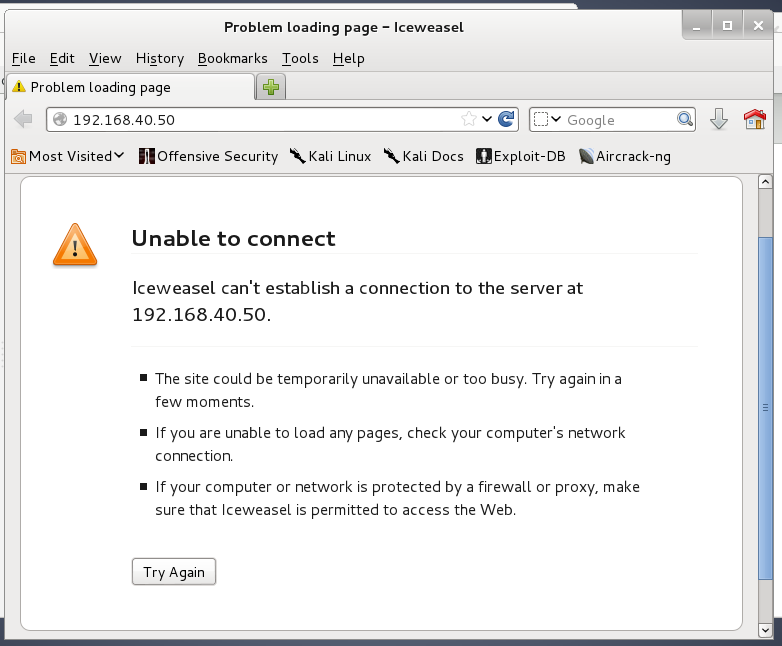
\includegraphics[width=16cm]{img/SYNFloodResult.png}\par

% Explanation of the result of the attack
\subsubsection{Attacker's messages}

\begin{longtable}{|l|l|l|l|l|l|p{5cm}|}
\hline
\textbf{No.} & \textbf{Time} & \textbf{Source} & \textbf{Destination} & \textbf{Protocol} & \textbf{Length} & \textbf{Info} \\
\hline
\endhead
5 & 0.050246000 &  192.168.62.20 & 192.168.40.50 & TCP &  56 & 1024 $>$ netbios-ssn [SYN] Seq=0 Win=8192 Len=0 \\
\hline
10 & 0.050727000 &  192.168.62.20 & 192.168.40.50 & TCP &  62 & [TCP Out-Of-Order] 1024 $>$ netbios-ssn [SYN] Seq=0 Win=8192 Len=0 \\
\hline
11 & 0.050870000 &  192.168.40.50 & 192.168.62.20 & TCP &  62 & netbios-ssn $>$ 1024 [RST, ACK] Seq=1 Ack=1 Win=0 Len=0 \\
\hline
17 & 0.190458000 &  192.168.62.20 & 192.168.40.50 & TCP &  56 & blackjack $>$ netbios-ssn [SYN] Seq=0 Win=8192 Len=0 \\
\hline
22 & 0.191035000 &  192.168.62.20 & 192.168.40.50 & TCP &  62 & [TCP Out-Of-Order] blackjack $>$ netbios-ssn [SYN] Seq=0 Win=8192 Len=0 \\
\hline
23 & 0.191965000 &  192.168.40.50 & 192.168.62.20 & TCP &  62 & netbios-ssn $>$ blackjack [RST, ACK] Seq=1 Ack=1 Win=0 Len=0 \\
\hline
24 & 0.286732000 &  192.168.62.20 & 192.168.40.50 & TCP &  56 & cap $>$ netbios-ssn [SYN] Seq=0 Win=8192 Len=0 \\
\hline
29 & 0.287236000 &  192.168.62.20 & 192.168.40.50 & TCP &  62 & [TCP Out-Of-Order] cap $>$ netbios-ssn [SYN] Seq=0 Win=8192 Len=0 \\
\hline
30 & 0.287373000 &  192.168.40.50 & 192.168.62.20 & TCP &  62 & netbios-ssn $>$ cap [RST, ACK] Seq=1 Ack=1 Win=0 Len=0 \\
\hline
34 & 0.415509000 &  192.168.62.20 & 192.168.40.50 & TCP &  56 & 1027 $>$ netbios-ssn [SYN] Seq=0 Win=8192 Len=0 \\
\hline
39 & 0.416019000 &  192.168.62.20 & 192.168.40.50 & TCP &  62 & [TCP Out-Of-Order] 1027 $>$ netbios-ssn [SYN] Seq=0 Win=8192 Len=0 \\
\hline
40 & 0.416127000 &  192.168.40.50 & 192.168.62.20 & TCP &  62 & netbios-ssn $>$ 1027 [RST, ACK] Seq=1 Ack=1 Win=0 Len=0 \\
\hline
44 & 0.527603000 &  192.168.62.20 & 192.168.40.50 & TCP &  56 & 1028 $>$ netbios-ssn [SYN] Seq=0 Win=8192 Len=0 \\
\hline
49 & 0.528239000 &  192.168.62.20 & 192.168.40.50 & TCP &  62 & [TCP Out-Of-Order] 1028 $>$ netbios-ssn [SYN] Seq=0 Win=8192 Len=0 \\
\hline
50 & 0.528354000 &  192.168.40.50 & 192.168.62.20 & TCP &  62 & netbios-ssn $>$ 1028 [RST, ACK] Seq=1 Ack=1 Win=0 Len=0 \\
\hline
54 & 0.618450000 &  192.168.62.20 & 192.168.40.50 & TCP &  56 & solid-mux $>$ netbios-ssn [SYN] Seq=0 Win=8192 Len=0 \\
\hline
58 & 0.702446000 &  192.168.62.20 & 192.168.40.50 & TCP &  56 & 1030 $>$ netbios-ssn [SYN] Seq=0 Win=8192 Len=0 \\
\hline
61 & 0.846491000 &  192.168.62.20 & 192.168.40.50 & TCP &  56 & 1031 $>$ netbios-ssn [SYN] Seq=0 Win=8192 Len=0 \\
\hline
64 & 0.978671000 &  192.168.62.20 & 192.168.40.50 & TCP &  56 & 1032 $>$ netbios-ssn [SYN] Seq=0 Win=8192 Len=0 \\
\hline
69 & 0.980323000 &  192.168.62.20 & 192.168.40.50 & TCP &  62 & [TCP Out-Of-Order] 1032 $>$ netbios-ssn [SYN] Seq=0 Win=8192 Len=0 \\
\hline
72 & 1.102467000 &  192.168.62.20 & 192.168.40.50 & TCP &  56 & netinfo-local $>$ netbios-ssn [SYN] Seq=0 Win=8192 Len=0 \\
\hline
75 & 1.299810000 &  192.168.62.20 & 192.168.40.50 & TCP &  56 & activesync $>$ netbios-ssn [SYN] Seq=0 Win=8192 Len=0 \\
\hline
78 & 1.406653000 &  192.168.62.20 & 192.168.40.50 & TCP &  56 & mxxrlogin $>$ netbios-ssn [SYN] Seq=0 Win=8192 Len=0 \\
\hline
81 & 1.550513000 &  192.168.62.20 & 192.168.40.50 & TCP &  56 & nsstp $>$ netbios-ssn [SYN] Seq=0 Win=8192 Len=0 \\
\hline
86 & 1.551117000 &  192.168.62.20 & 192.168.40.50 & TCP &  62 & [TCP Out-Of-Order] nsstp $>$ netbios-ssn [SYN] Seq=0 Win=8192 Len=0 \\
\hline
87 & 1.551240000 &  192.168.40.50 & 192.168.62.20 & TCP &  62 & netbios-ssn $>$ nsstp [RST, ACK] Seq=1 Ack=1 Win=0 Len=0 \\
\hline
91 & 1.631353000 &  192.168.62.20 & 192.168.40.50 & TCP &  56 & ams $>$ netbios-ssn [SYN] Seq=0 Win=8192 Len=0 \\
\hline
94 & 1.775418000 &  192.168.62.20 & 192.168.40.50 & TCP &  56 & mtqp $>$ netbios-ssn [SYN] Seq=0 Win=8192 Len=0 \\
\hline
97 & 1.910714000 &  192.168.62.20 & 192.168.40.50 & TCP &  56 & sbl $>$ netbios-ssn [SYN] Seq=0 Win=8192 Len=0 \\
\hline
100 & 2.030476000 &  192.168.62.20 & 192.168.40.50 & TCP &  56 & netarx $>$ netbios-ssn [SYN] Seq=0 Win=8192 Len=0 \\
\hline
105 & 2.223798000 &  192.168.62.20 & 192.168.40.50 & TCP &  56 & danf-ak2 $>$ netbios-ssn [SYN] Seq=0 Win=8192 Len=0 \\
\hline
110 & 2.224472000 &  192.168.62.20 & 192.168.40.50 & TCP &  62 & [TCP Out-Of-Order] danf-ak2 $>$ netbios-ssn [SYN] Seq=0 Win=8192 Len=0 \\
\hline
\multicolumn{7}{l}{\textit{*****************}} \\ \\
\hline
1132 & 56.064211000 & 192.168.62.20 & 192.168.40.50 & TCP &  56 & nicelink $>$ http [SYN] Seq=0 Win=8192 Len=0 \\
\hline
1136 & 56.135107000 & 192.168.62.20 & 192.168.40.50 & TCP &  56 & cnrprotocol $>$ http [SYN] Seq=0 Win=8192 Len=0 \\
\hline
1139 & 56.223321000 & 192.168.62.20 & 192.168.40.50 & TCP &  56 & sunclustermgr $>$ http [SYN] Seq=0 Win=8192 Len=0 \\
\hline
1149 & 56.326467000 & 192.168.62.20 & 192.168.40.50 & TCP &  56 & rmiactivation $>$ http [SYN] Seq=0 Win=8192 Len=0 \\
\hline
1152 & 56.590463000 & 192.168.62.20 & 192.168.40.50 & TCP &  56 & mctp $>$ http [SYN] Seq=0 Win=8192 Len=0 \\
\hline
1154 & 56.666537000 & 192.168.62.20 & 192.168.40.50 & TCP &  56 & pt2-discover $>$ http [SYN] Seq=0 Win=8192 Len=0 \\
\hline
1157 & 56.862634000 & 192.168.62.20 & 192.168.40.50 & TCP &  56 & adobeserver-1 $>$ http [SYN] Seq=0 Win=8192 Len=0 \\
\hline
1160 & 56.974430000 & 192.168.62.20 & 192.168.40.50 & TCP &  56 & adobeserver-2 $>$ http [SYN] Seq=0 Win=8192 Len=0 \\
\hline
1163 & 57.050435000 & 192.168.62.20 & 192.168.40.50 & TCP &  56 & xrl $>$ http [SYN] Seq=0 Win=8192 Len=0 \\
\hline
1166 & 57.166421000 & 192.168.62.20 & 192.168.40.50 & TCP &  56 & ftranhc $>$ http [SYN] Seq=0 Win=8192 Len=0 \\
\hline
1171 & 57.166989000 & 192.168.62.20 & 192.168.40.50 & TCP &  62 & [TCP Out-Of-Order] ftranhc $>$ http [SYN] Seq=0 Win=8192 Len=0 \\
\hline
1172 & 57.167114000 & 192.168.40.50 & 192.168.62.20 & TCP &  62 & http $>$ ftranhc [RST, ACK] Seq=1 Ack=1 Win=0 Len=0 \\
\hline
1186 & 57.343848000 & 192.168.62.20 & 192.168.40.50 & TCP &  56 & isoipsigport-1 $>$ http [SYN] Seq=0 Win=8192 Len=0 \\
\hline
1190 & 57.492962000 & 192.168.62.20 & 192.168.40.50 & TCP &  56 & isoipsigport-2 $>$ http [SYN] Seq=0 Win=8192 Len=0 \\
\hline
1193 & 57.647757000 & 192.168.62.20 & 192.168.40.50 & TCP &  56 & ratio-adp $>$ http [SYN] Seq=0 Win=8192 Len=0 \\
\hline
1196 & 57.775299000 & 192.168.62.20 & 192.168.40.50 & TCP &  56 & kpop $>$ http [SYN] Seq=0 Win=8192 Len=0 \\
\hline
1201 & 57.775889000 & 192.168.62.20 & 192.168.40.50 & TCP &  62 & [TCP Out-Of-Order] kpop $>$ http [SYN] Seq=0 Win=8192 Len=0 \\
\hline
1202 & 57.776027000 & 192.168.40.50 & 192.168.62.20 & TCP &  62 & http $>$ kpop [RST, ACK] Seq=1 Ack=1 Win=0 Len=0 \\
\hline
1206 & 57.918417000 & 192.168.62.20 & 192.168.40.50 & TCP &  56 & webadmstart $>$ http [SYN] Seq=0 Win=8192 Len=0 \\
\hline
1209 & 58.007475000 & 192.168.62.20 & 192.168.40.50 & TCP &  56 & lmsocialserver $>$ http [SYN] Seq=0 Win=8192 Len=0 \\
\hline
1212 & 58.093061000 & 192.168.62.20 & 192.168.40.50 & TCP &  56 & icp $>$ http [SYN] Seq=0 Win=8192 Len=0 \\
\hline
1215 & 58.174390000 & 192.168.62.20 & 192.168.40.50 & TCP &  56 & ltp-deepspace $>$ http [SYN] Seq=0 Win=8192 Len=0 \\
\hline
1220 & 58.174972000 & 192.168.62.20 & 192.168.40.50 & TCP &  62 & [TCP Out-Of-Order] ltp-deepspace $>$ http [SYN] Seq=0 Win=8192 Len=0 \\
\hline
1221 & 58.175934000 & 192.168.40.50 & 192.168.62.20 & TCP &  62 & http $>$ ltp-deepspace [RST, ACK] Seq=1 Ack=1 Win=0 Len=0 \\
\hline
1224 & 58.255786000 & 192.168.62.20 & 192.168.40.50 & TCP &  56 & mini-sql $>$ http [SYN] Seq=0 Win=8192 Len=0 \\
\hline
1241 & 59.223890000 & 192.168.48.9 &  192.168.40.50 & ICMP & 84 & Destination unreachable (Host unreachable) \\
\hline
1242 & 59.223893000 & 192.168.48.9 &  192.168.40.50 & ICMP & 84 & Destination unreachable (Host unreachable) \\
\hline
1243 & 59.223897000 & 192.168.48.9 &  192.168.40.50 & ICMP & 84 & Destination unreachable (Host unreachable) \\
\hline
\multicolumn{7}{l}{\textit{*******Legit requests are denied: *******}} \\ \\
\hline
1249 & 63.565147000 & 192.168.62.60 & 192.168.40.50 & TCP &  76 & 33648 $>$ http [SYN] Seq=0 Win=29200 Len=0 MSS=1460 SACK\_PERM=1 TSval=1433332 TSecr=0 WS=128 \\
\hline
1254 & 63.565751000 & 192.168.62.60 & 192.168.40.50 & TCP &  76 & [TCP Out-Of-Order] 33648 $>$ http [SYN] Seq=0 Win=29200 Len=0 MSS=1460 SACK\_PERM=1 TSval=1433332 TSecr=0 WS=128 \\
\hline
1255 & 63.565889000 & 192.168.40.50 & 192.168.62.60 & TCP &  62 & http $>$ 33648 [RST, ACK] Seq=1 Ack=1 Win=0 Len=0 \\
\hline
1260 & 63.566309000 & 192.168.40.50 & 192.168.62.60 & TCP &  62 & http $>$ 33648 [RST, ACK] Seq=1 Ack=1 Win=0 Len=0 \\
\hline
1261 & 63.566395000 & 192.168.62.60 & 192.168.40.50 & TCP &  76 & 33649 $>$ http [SYN] Seq=0 Win=29200 Len=0 MSS=1460 SACK\_PERM=1 TSval=1433332 TSecr=0 WS=128 \\
\hline
1266 & 63.566843000 & 192.168.62.60 & 192.168.40.50 & TCP &  76 & [TCP Out-Of-Order] 33649 $>$ http [SYN] Seq=0 Win=29200 Len=0 MSS=1460 SACK\_PERM=1 TSval=1433332 TSecr=0 WS=128 \\
\hline
1267 & 63.566916000 & 192.168.40.50 & 192.168.62.60 & TCP &  62 & http $>$ 33649 [RST, ACK] Seq=1 Ack=1 Win=0 Len=0 \\
\hline
1272 & 63.567300000 & 192.168.40.50 & 192.168.62.60 & TCP &  62 & http $>$ 33649 [RST, ACK] Seq=1 Ack=1 Win=0 Len=0 \\
\hline
1273 & 63.567495000 & 192.168.62.60 & 192.168.40.50 & TCP &  76 & 33650 $>$ http [SYN] Seq=0 Win=29200 Len=0 MSS=1460 SACK\_PERM=1 TSval=1433332 TSecr=0 WS=128 \\
\hline
1278 & 63.567886000 & 192.168.62.60 & 192.168.40.50 & TCP &  76 & [TCP Out-Of-Order] 33650 $>$ http [SYN] Seq=0 Win=29200 Len=0 MSS=1460 SACK\_PERM=1 TSval=1433332 TSecr=0 WS=128 \\
\hline
1279 & 63.567886000 & 192.168.40.50 & 192.168.62.60 & TCP &  62 & http $>$ 33650 [RST, ACK] Seq=1 Ack=1 Win=0 Len=0 \\
\hline
1284 & 63.568524000 & 192.168.40.50 & 192.168.62.60 & TCP &  62 & http $>$ 33650 [RST, ACK] Seq=1 Ack=1 Win=0 Len=0 \\
\hline
1285 & 63.568636000 & 192.168.62.60 & 192.168.40.50 & TCP &  76 & 33651 $>$ http [SYN] Seq=0 Win=29200 Len=0 MSS=1460 SACK\_PERM=1 TSval=1433332 TSecr=0 WS=128 \\
\hline
1290 & 63.569031000 & 192.168.62.60 & 192.168.40.50 & TCP &  76 & [TCP Out-Of-Order] 33651 $>$ http [SYN] Seq=0 Win=29200 Len=0 MSS=1460 SACK\_PERM=1 TSval=1433332 TSecr=0 WS=128 \\
\hline
1291 & 63.569101000 & 192.168.40.50 & 192.168.62.60 & TCP &  62 & http $>$ 33651 [RST, ACK] Seq=1 Ack=1 Win=0 Len=0 \\
\hline
1296 & 63.569445000 & 192.168.40.50 & 192.168.62.60 & TCP &  62 & http $>$ 33651 [RST, ACK] Seq=1 Ack=1 Win=0 Len=0 \\
\hline
\end{longtable}


In this case the attacker (PC2) is sending multiple SYN flags to the victim and in the last part of the messages is possible to see that even legit requests are denied.\par

% Method recommended to protect the Network against such an attack
\subsubsection{How to protect the network}
The possible solutions for prevent SYN Flood is to increase the backlog for TCP and to enable the syn cookies. Syn cookies are use to prevent syn flood by enlarging the SYN queue when it fills up. Now the server keeps responding with [SYN,ACK] but the server discards the SYN queue entries. When the server received an ACK flag it is able to reconstruct the SYN queue entry using informations encoded in TCP sequence number.\par
Another solution is to use a firewall. Some implementations of the firewall could be:\\
\begin{lstlisting}
iptables -A INPUT -p tcp -m state --state NEW
    -m recent --update --seconds 60 --hitcount 20 -j DROP

iptables -A INPUT -p tcp -m state --state NEW
    -m recent --set -j ACCEPT
\end{lstlisting}
In this way we limit the SYN request up to 20 per minute and we prevent the SYN flood. This is not best way to protect the network from Syn flood because in we can also drop legit requests coming from a network behind a nat.\par
Another implementation of the firewall could be:\\
\begin{lstlisting}
iptables -t mangle -I PREROUTING -p tcp -m tcp --dport 80
    -m state --state NEW -m tcpmss ! --mss 536:65535 -j DROP
\end{lstlisting}
This rule checks 2 things. The first one is that the TCP Header contains the maximum size that the host wants to allow (hping, common attacking tool, doesn’t set this parameter by default). The second one is to check the port of the clients are in the range from 536 to 35535.\par
